\documentclass[english,a4paper]{article}

\usepackage{graphicx}
\usepackage[english]{babel}
\usepackage[latin1]{inputenc}
\usepackage{amsmath}
\usepackage{moreverb}
\usepackage{psfrag}
\usepackage[ps2pdf]{hyperref}
\usepackage{listings}
\usepackage{macros}


\graphicspath{{Figures/}}

\setcounter{tocdepth}{2}

\newcommand{\MBSim}{\href{http://mbsim.berlios.de}{\textsf{MBSim}}}
\newcommand{\AMVis}{\href{http://www.amm.mw.tum.de}{\textsf{AMVis}}}
\newcommand{\FMatVec}{\href{http://fmatvec.berlios.de}{\textsf{FMatVec}}}
\newcommand{\HDF}{\href{http://www.hdfgroup.org/HDF5/}{\textsf{HDF5}}}

% document
\begin{document}
\title{\MBSim{} - A Kind (Of) Introduction}
\author{by \MBSim{} Development Team\\
  Mathias Bachmayer\\
  Bastian Esefeld\\
  Martin F\"org\\
  Markus Friedrich\\
  Robert Huber\\
  Thorsten Schindler\\
  Markus Schneider\\
  Roland Zander}
\date{24.04.2009}
\maketitle

\begin{abstract}
  This manual explains how to install \MBSim{} and introduces easy examples.
\end{abstract}

\noindent\hrulefill
\tableofcontents

%%%%%%%%%%%%%%%%%%%%%%%%%%%%%%%%%%%%%%%%%%%%%%%%%%%%%%%%%%%%%%%%%%%%%%%%%%%%%%%%
%%%%%%%%%%%%%%%%%%%%%%%%%%%%%%%%%%%%%%%%%%%%%%%%%%%%%%%%%%%%%%%%%%%%%%%%%%%%%%%%

\section{Introduction}
\MBSim{} is a simulation tool to analyse the dynamic phenomenons of dynamical systems. Its root is the modelling of nonsmooth multibody system explaining the program name \MBSim{}. The mathematical background has been developed over years at the Institute of Applied Mechanics of the Technische Universit\"at M\"unchen. The last summary concerning rigid body dynamics was given in the PhD thesis and the lecture of Martin F\"org~\cite{Foer09,Foer07}. The PhD thesis of Roland Zander~\cite{Zan09} introduces the theory of flexible bodies. Ref.~\cite{Zan08} shows an overview about the research at the institute in the last decades concerning nonsmooth mechanics. This reference also includes simulation results of academic and industrial examples. Extensions regarding hydraulics and signal processing as well as parallelisation and cosimulation are unique in the field of nonsmooth dynamical systems.\par
The goal of this introduction is to motivate the use of \MBSim{}. It shows the installation of the necessary program parts, describes basically its components and program flow and gives some examples. You find it in the Download section of the \MBSim{} webpage, where you can also find binary releases for Linux and Windows as well as~\cite{Zan08}. For more information, e.g. Doxygen description and current build status, visit the {\href{http://www4.amm.mw.tu-muenchen.de:8080/mbsim-env/}{\textsf{Central Build System}}}.


\section{Installation}
This section summarizes the necessary steps to install \MBSim{}.

%%------------------------------------------------------------ SUBSECTION ---------------------
\subsection{Where To Find the Source Code}
The source code of \MBSim{} together with some examples, the necessary \FMatVec{} library, a \HDF{} wrapper for output and the visualisation program \OpenMBV{} can be found at \url{www.berlios.de} using subversion code administration\footnote{SVN Quick Reference Card: \url{http://www.cs.put.poznan.pl/csobaniec/edu/svn-refcard.pdf}}. Further, one needs \HDF{} from \url{http://www.hdfgroup.org}. Everything is placed under \href{http://www.gnu.org/licenses/lgpl.html}{LGPL}\footnote{see file~\texttt{COPYING} in the root directory of the specific source code}.\par
In the following it is assumed, that a directory~\texttt{MBSim} and a directory \texttt{MBSim/Install} has been created in the \texttt{\$HOME} path of the Linux operating system. 

%%------------------------------------------------------------ SUBSECTION ---------------------
\subsection{Installation Procedures}
All projects depend on PKG package administration. That is why the file \texttt{\$HOME/.bashrc} has to be extended with
\begin{verbatim}
 export PKG_CONFIG_PATH=
        "$HOME/MBSim/Install/lib/pkgconfig/:$PKG_CONFIG_PATH"
 export LD_LIBRARY_PATH=
        "$HOME/MBSim/Install/lib/:$LD_LIBRARY_PATH"
\end{verbatim}
For the installation of the specific projects always the same \emph{procedures} have to be applied. They are summarised in the following.

\subsubsection{Installation}
\begin{itemize}
	\item \textsc{automake}:
	\begin{itemize}
		\item[] \begin{verbatim}aclocal\end{verbatim}
		\item[] \texttt{autoheader}
		\item[] \texttt{autoconf}
		\item[] \begin{verbatim}libtoolize -c --force\end{verbatim}
		\item[] \begin{verbatim}automake -a -c --force\end{verbatim}
	\end{itemize}
	\item \textsc{configure}: 
	\begin{itemize}
		\item[] \begin{verbatim}./configure --prefix=$HOME/MBSim/Install F77=gfortran \end{verbatim}
        \item[] possibly FLAGS for debug information
		        \begin{verbatim} CFLAGS="-g3 -O0" CXXFLAGS="-g3 -O0" F77FLAGS="-g3 -O0" FFLAGS="-g3 -O0" \end{verbatim}
		\item[] possibly project depending FLAGS
	\end{itemize}
	\item \textsc{install}
	\begin{itemize}	
		\item \begin{verbatim}make\end{verbatim}
		\item \begin{verbatim}make install\end{verbatim}
	\end{itemize}
\end{itemize}
All procedures belong to the GNU-Build-System (cf.~Sec.~\ref{sec:gnu}).\par
It is reasonable to write an executable script file invoking the procedures.

\subsubsection{Reinstallation}
The procedure \textsc{reinstall}
\begin{verbatim}
 ./config.status --recheck
 ./config.status
 make clean
 make install
\end{verbatim}
newly installs a project.\par
For restoring a not-configured version of the project
\begin{verbatim}
 make maintainer-clean
\end{verbatim}
is used. After that \textsc{configure} has to be invoked again.

\subsubsection{Uninstallation}
For uninstall
\begin{verbatim}
 make clean
 make uninstall
\end{verbatim}
has to be called in all directories.

%%------------------------------------------------------------ SUBSECTION ---------------------
\subsection{\FMatVec{}}
\FMatVec{} is a library for fast matrix-vector evaluations based on LAPack with the possibility to use ATLAS, which is faster for large system dimensions because of internal parallelisation.\\
For the installation the following instructions have to be completed:
\begin{verbatim}
 cd $HOME/MBSim
 svn checkout http://svn.berlios.de/svnroot/repos/fmatvec/trunk fmatvec
 cd $HOME/MBSim/fmatvec
\end{verbatim}
Continue with the procedure \textsc{automake}.\par
Then, the procedure \textsc{configure} is used selecting the FLAGS
\begin{verbatim}
 --with-blas-lib-prefix=PFX (prefix, where the BLAS lib is
     installed, when ATLAS is not used)
 --with-lapack-lib-prefix=PFX (prefix, where the LAPACK lib is
     installed, when ATLAS is not used)
\end{verbatim}
if LAPack is not located in a standard search path and selecting
\begin{verbatim}
 --enable-atlas (use ATLAS)
 --with-atlas-inc-prefix=PFX (prefix, where the ATLAS includes 
     are installed, when ATLAS is used)
 --with-atlas-lib-prefix=PFX (prefix, where the ATLAS libs are
     installed, when ATLAS is used)
\end{verbatim}
if ATLAS should be used instead of LAPack. The FLAGS
\begin{verbatim}
 --with-allocator-class=__gnu_cxx::new_allocator
 --with-allocator-header=ext/new_allocator.h
\end{verbatim}
are necessary to use a standard thread-safe memory allocator instead of the \FMatVec{} built-in allocator.\par
The code can be compiled and installed with a Doxygen HTML class documentation by \texttt{make doc} and the procedure \textsc{install}.

%%------------------------------------------------------------ SUBSECTION ---------------------
\subsection{\HDF}
\HDF{} is a hierarchical data format enabling the effective administration of plot and visualisation data. It can be downloaded as source code from \url{http://www.hdfgroup.org/HDF5/} with at least version 1.8.2.\par
Extract the source archive to \texttt{\$HOME/MBSim/hdf5}.\par
Change to \texttt{\$HOME/MBSim/hdf5}.\par
Use the procedure \textsc{configure} with the additional FLAG
\begin{verbatim}
 --enable-cxx
\end{verbatim}
Compilation is done with the procedure \textsc{install}.\par
A \HDF{} wrapper makes it possible to use \HDF{} very easily. It is available by
\begin{verbatim}
 cd $HOME/MBSim
 svn checkout http://svn.berlios.de/svnroot/repos/hdf5serie/trunk HDF5Serie
\end{verbatim}
For having \MBSim{} creating \HDF{} files invoke
\begin{verbatim}
 cd $HOME/MBSim/HDF5Serie/hdf5serie
\end{verbatim}
as well as the procedures \textsc{automake, configure}, \texttt{make doc} and \textsc{install} for installation and creation of a Doxygen HTML class documentation.\par
For convenient plotting of \HDF{} files it is assumed that Qwt with version 5 or newer is installed (cf. Sec.~\ref{sec:third_party}).\par
Invoke 
\begin{verbatim}
 ssh diesel (only at the institute)
 export PKG_CONFIG_PATH=/home/OpenMBV/local/lib/pkgconfig:
    $HOME/MBSim/Install/lib/pkgconfig (only at the institute)
 cd $HOME/MBSim/HDF5Serie/h5plotserie
\end{verbatim}
as well as the procedures \textsc{automake, configure}, \texttt{make doc} and \textsc{install} for installation and creation of a Doxygen HTML class documentation. Then,
\begin{verbatim}
 exit (only at the institute)
\end{verbatim}
Last, \texttt{.bashrc} can be extended with
\begin{verbatim}
alias h5lsserie="$HOME/MBSim/Install/bin/h5lsserie"
alias h5dumpserie="$HOME/MBSim/Install/bin/h5dumpserie"
alias h5plotserie="$HOME/MBSim/Install/bin/h5plotserie"
\end{verbatim}
to gain overall access to the commands \texttt{h5lsserie}, \texttt{h5dumpserie} and \texttt{h5plotserie}.

%%------------------------------------------------------------ SUBSECTION ---------------------
\subsection{\OpenMBV{}}
\OpenMBV{} visualises \MBSim{} simulations using XML and \HDF{} in a coinciding hierarchical structure. The installation consists of three steps: first the XML utils have to be installed, then \OpenMBV{} has to be build for visualisation, and third \MBSim{} needs \textsf{OpenMBV-C++Interface} to create standard data for \OpenMBV{} using C++ programs. The source code is available by
\begin{verbatim}
 cd $HOME/MBSim
 svn checkout http://svn.berlios.de/svnroot/repos/openmbv/trunk OpenMBV
\end{verbatim}

\subsubsection{XML Utils}
It is assumed that Octave with version 3.0 or newer is installed (cf. Sec.~\ref{sec:third_party}).\par
Then,
\begin{verbatim}
 cd $HOME/MBSim/OpenMBV/mbxmlutils
\end{verbatim} 
and use the procedures \textsc{automake}, \textsc{configure} with FLAG \texttt{\-\-with-mkoctfile-path} (\texttt{Octave/bin}) and \textsc{install} for installation of an independent XML preprocessor to parse and validate hierarchical XML-files with Octave code.

\subsubsection{\OpenMBV{}}
There is a static Linux binary available at \url{www.berlios.de} being updated from time to time.\par
For the installation of a static visualisation using always the newest source files it is assumed that
\begin{itemize}
\item Coin3d with version 3 or newer 
\item hdf5 with version 1.8.2 or newer 
\item Qt with version 4.4 or newer 
\item HDF5Serie 
\item SoQt with version 1.4.1 or newer 
\item Qwt with version 5 or newer 
\end{itemize}
is installed (cf. Sec.~\ref{sec:third_party}).\par
With
\begin{verbatim}
 ssh diesel (only at the institute)
 export PKG_CONFIG_PATH=/home/OpenMBV/local/lib/pkgconfig:
    $HOME/MBSim/Install/lib/pkgconfig (only at the institute)
 cd $HOME/MBSim/OpenMBV/openmbv
\end{verbatim} 
and the procedures \textsc{automake, configure}, \texttt{make doc} and \textsc{install} a static build of the viewer together with an Doxygen HTML class documentation completes the installation. Then,
\begin{verbatim}
 exit (only at the institute)
\end{verbatim}
Last, \texttt{.bashrc} can be extended with
\begin{verbatim}
 alias openmbv="$HOME/MBSim/Install/bin/openmbv"
\end{verbatim}
to gain overall access to the command \texttt{openmbv}, which should be used only locally because of network protocols not providing the necessary X.org requirements.

\subsubsection{OpenMBV-C++Interface}
It is assumed that 
\begin{itemize}
\item hdf5 with version 1.8.2 or newer
\item HDF5Serie 
\end{itemize}
is installed.\par
Invoke
\begin{verbatim}
 cd $HOME/MBSim/OpenMBV/openmbvcppinterface
\end{verbatim} 
and the procedures \textsc{automake, configure}, \texttt{make doc} and \textsc{install} for installation and creation of a Doxygen HTML class documentation. 

%%------------------------------------------------------------ SUBSECTION ---------------------
\subsection{\MBSim}
Necessary for the installation of \MBSim{} are
\begin{itemize}
\item \FMatVec{}
\item \OpenMBV{}-C++-Interface
\end{itemize}
For installation of \MBSim{} one types
\begin{verbatim}
 cd $HOME/MBSim
 svn checkout http://svn.berlios.de/svnroot/repos/mbsim/trunk mbsim
 cd $HOME/MBSim/mbsim/kernel
\end{verbatim}
Invoke the procedures \textsc{automake, configure}, \texttt{make doc} and \textsc{install} to install the basic module and to create a Doxygen HTML class documentation. In
\begin{verbatim}
$HOME/MBSim/mbsim/kernel/xmldoc
\end{verbatim}
invoke \textsc{install} for an XML documentation in \texttt{\$HOME/MBSim/Install/share/mbxmlutils/doc}.
\begin{verbatim}
 cd $HOME/MBSim/mbsim/modules/mbsimControl
\end{verbatim}
Invoke the procedures \textsc{automake, configure}, \texttt{make doc} and \textsc{install} to install the signal processing and control module and to create a Doxygen HTML class documentation. In 
\begin{verbatim}
$HOME/MBSim/mbsim/modules/mbsimControl/xmldoc
\end{verbatim}
invoke \textsc{install} for an XML documentation in \texttt{\$HOME/MBSim/Install/share/mbxmlutils/doc}.
\begin{verbatim}
 cd $HOME/MBSim/mbsim/modules/mbsimHydraulics
\end{verbatim}
Invoke the procedures \textsc{automake, configure}, \texttt{make doc} and \textsc{install} to install the hydraulics module and to create a Doxygen HTML class documentation. In 
\begin{verbatim}
$HOME/MBSim/mbsim/modules/mbsimHydraulics/xmldoc
\end{verbatim}
invoke \textsc{install} for an XML documentation in \texttt{\$HOME/MBSim/Install/share/mbxmlutils/doc}.
\begin{verbatim}
 cd $HOME/MBSim/mbsim/modules/mbsimElectronics
\end{verbatim}
Invoke the procedures \textsc{automake, configure}, \texttt{make doc} and \textsc{install} to install the electronics module and to create a Doxygen HTML class documentation. 
\begin{verbatim}
 cd $HOME/MBSim/mbsim/modules/mbsimPowerTrain
\end{verbatim}
Invoke the procedures \textsc{automake, configure}, \texttt{make doc} and \textsc{install} to install the module for gears and to create a Doxygen HTML class documentation. 
\begin{verbatim}
 cd $HOME/MBSim/mbsim/mbsimxml
\end{verbatim}
Invoke the procedures \textsc{automake, configure} and \textsc{install} to install the XML module which contains an executable to invoke the preprocessor and after that evaluate the resulting flat structure. In
\begin{verbatim}
$HOME/MBSim/mbsim/mbsimxml/xmldoc
\end{verbatim}
invoke \textsc{install} for an XML documentation in \texttt{\$HOME/MBSim/Install/share/mbxmlutils/doc}.

%%------------------------------------------------------------ SUBSECTION ---------------------
\subsection{MBSimAddOns}
At the institute further modules can be found in \texttt{MBSimAddOn}: mechanical components~(\texttt{mbsimMechAdd}), hydraulic components~(\texttt{mbsimHydraulics}), and an interface for co-simulationen~(\texttt{mbsimCosim}). For installation one types
\begin{verbatim}
 svn checkout http://zeiss/repos/SVN--rep//AM-software/mbsimAddOn/trunk mbsimAddOn
\end{verbatim}
in directory \texttt{MBSim}. Then one uses the procedures \textsc{automake, configure} and \textsc{install} in the subdirectories of \texttt{MBSim/mbsimAddOn}.

%%------------------------------------------------------------ SUBSECTION ---------------------
\subsection{\MBSim Examples}
The examples are used for testing successful installation. There are two possibilities:
\begin{enumerate}
\item Change to the specific directory \texttt{\$HOME/MBSim/mbsim/examples/*} and type \texttt{make} to create an executable. The simulation starts with the command~\texttt{./main}. The results are visualised with the command~\texttt{openmbv} and plotted with~\texttt{h5plotserie} (cf.~Sec.~\ref{sec:plot}).
\item Use the script \texttt{./runexamples.sh install} in \texttt{\$HOME/MBSim/mbsim/examples} to install reference files. Then \texttt{./runexamples.sh} compiles, runs and tests each example. See \texttt{./runexamples.sh -h} for additional information.
\end{enumerate}


\section{\MBSim - Program Overview}
\MBSim{} is written in the object-orientated programming language C++. 

Fig.~\ref{fig:objects} shows a class diagram.
\begin{figure}
	\centering
  	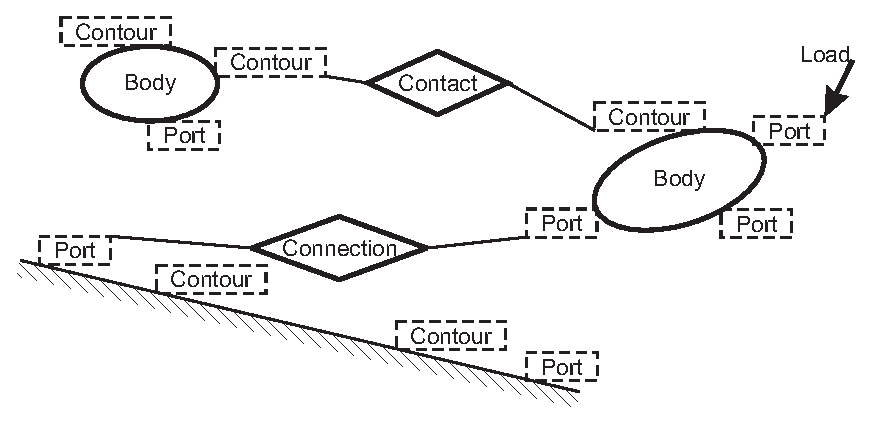
\includegraphics[width=12cm]{Figures/objectorientationMBSim.eps} % TODO
  	\caption{object structure in \MBSim}
  	\label{fig:objects}
\end{figure}

\subsection{Description of the Components}
The following classes can be used for modelling and simulating dynamical systems in \MBSim{}.

\subsubsection{Frames}

\subsubsection{Rigid Bodies}
To describe the kinematics and the update of further frames at rigid bodies a body-fixed frame has to be defined in \texttt{RigidBody} based on a predefined frame \texttt{"C"} in the centre of gravity. The frame for kinematics is updated with respect to a reference frame and its individual degree of freedom or its constrained relative motion. Both absolute and relative kinematical structures are canonically given by this frame recursion depending on the properties of the reference. The drawback of this general description is a time-dependent mass-matrix. A constant mass evaluation can be enforced by a boolean \texttt{"cb"}.\\
If there is a frame given tree structure a \texttt{Tree} for the kinematical evaluations is defined automatically.
%In jedem Fall sind Masse (\emph{setMass}), Tr\"agheitstensor bez. dem Bezugspunkt (\emph{setInertia}), generalisierte Koordinaten (\emph{setJT}, \emph{setJR}), evtl. Anfangsverformungen (\emph{setWrOK0}, \emph{setAWK0}) und \AMVis{}-Darstellungen (\emph{setAMVisBody}) anzugeben und die K\"orper dem MKS hinzuzuf\"ugen (\emph{addObject}). Auch ganze MKS k\"onnen als Slave einem Master-MKS hinzugef\"ugt werden.

\subsubsection{Flexible Bodies}
The equations of motion of a \texttt{FlexibleBody} is at the moment always derived with respect to a stationary frame. So, flexible bodies can only be used as root but not as leave in a recursive tree structure. The following flexible bodies are available. 

\begin{itemize}
%\item \emph{BodyFlexible1s01Torsion}
%\item \emph{BodyFlexible1s21ANCF} 2D-Balken mit Absolute Nodal Coordinate Formulation
\item[] \texttt{BodyFlexible1s21RCM}\\
  planar beam using redundant coordinate methode with three coordinates per finite element node, translation  $x$, $y$ and rotation $\gamma$, as well as two additional bending deflections $c_1$, $c_2$
\item[] \texttt{BodyFlexible1s33RCM}\\
  spatial beam using redundant coordinate methode with six coordinates per finite element node, translation  $x$, $y$, $z$ and reversed Cardan rotation $\alpha$, $\beta$, $\gamma$, as well as four additional bending deflections $c_1$, $c_2$, $c_3$, $c_4$
%\item \emph{BodyFlexible1s23BTA} Biege-Torsions-Welle (5-Koordinaten pro Knoten $\alpha$, $y$, $\gamma$, $z$, $\beta$ im jeweils mit $\alpha$ mitdrehenden KOSY)
%\item \emph{BodyFlexibleLinearExternal}
\end{itemize}
%F\"ur die RCM-Modelle sowie die Biege-Torsions-Welle kann eine \AMVis-Darstellung
%(\emph{createAMVisBody}) aktiviert werden. Die Finiten Elemente selbst basieren im Fall von \emph{BodyFlexible1s21RCM}, \emph{BodyFlexible1s23BTA} und \emph{BodyFlexibleLinearExternal} auf einem neugeschaffenem Interface \emph{DiscretizationInterface} zur einheitlichen Darstellung.
%
%\subsubsection{Joints}
%Verbindungen werden ohne Reibung \"uber Ports (\emph{addPort}, \emph{connect}) an K\"orper bez. an die Umgebung angeschlossen. Dann ist auszuw\"ahlen, ob eine flexible Verbindung (\emph{ConnectionFlexible}) oder eine Starrk\"orperverbindung (\emph{ConnectionRigid}) zwischen K\"orpern oder eine externe Erregung (\emph{Load}) zur Modellierung verwendet werden soll. Der Freiheitsgrad der Verbindung wird \"uber \emph{setForceDirection} bez. \emph{setMomentDirection} angegeben. Dem MKS wird eine Verbindung anschlie"send \"uber \emph{addLink} mitgeteilt. \"Uber \emph{Link} kann auch eine Visualisierung der Verbindungskr\"afte (\emph{Arrow}) und der Kopplung selbst zugeschaltet werden; hierbei ist es m\"oglich zwischen einer Einheitenumrechnung und einer L\"angenvisualisierung zu unterscheiden (\emph{setScaleFactor}, \emph{setArrowHead}, \emph{setDiameter}), sowie den Partner f\"ur das Pfeilende festzulegen. Bei \emph{Load} wird mit \emph{setSignal} eine benutzerspezifische Funktion\footnote{\emph{UserFunction} gibt es bereits mit harmonischen (\emph{FuncHarmonic}), linearen Verlauf (\emph{FuncLinear}), oder auch als mehrdimensionale st\"uckweise Polynominterpolation (\emph{MDPPolynom})} vorgegeben.
%
\subsubsection{Contacts and Impacts}
Contacts and impacts are managed by \texttt{Contact}.\par 
The relative kinematics is defined between \texttt{Contour} classes. Thereby kinematically there might be a finite number of possible contact points; for the evaluation of force laws a decision rule has to be implemented. On velocity level the contact kinematics is independent of the specific contour. For the calculations on position level the following contours are available.
\begin{itemize}
\item[] \texttt{Point}\\
    most primitive rigid contour
\item[] \texttt{Plane}\\
    affine two dimensional surface
\item[] \texttt{Sphere}\\
    two dimensional sphere
\item[] \texttt{FlexibleBand}\\
    flexible contour describing a band in a certain distance and direction of a neutral fibre
\end{itemize}

Available contact kinematics on position level:
\begin{itemize}
\item[] \texttt{PointPlane}
\item[] \texttt{PointFlexibleBand}
\item[] \texttt{SpherePlane}
\end{itemize}

Concerning the constitutive laws it is distinguished between contact laws on acceleration and impact laws on velocity level. Further, both flexible and rigid laws in normal and tangential direction are available.\footnote{Modelling hint: There are contradictions between energy conservation in normal direction and dissipation due to friction when combining these features.})\par

For modelling own contact kinematics and constitutive laws some conventions are important.
\begin{itemize}
\item accompanying contour trihedral\\
    the first column is the outward pointing normal, 
\end{itemize}

%Linie-Contour1s, Kugel-Ebene, Kugel-Kugel und Kugel-Kegelstumpf. Auch Erweiterungen
%k\"onnen \"uber die Definition neuer Konturen und zugeh\"origer Kontaktkinematiken
%(\emph{setContactKinematics}) definiert werden. Hierzu ben\"otigt eine Kontur die
%Parametrisierung einer nach innen gerichteten Normale, einer Tangente, einer Position,
%einer Geschwindigkeit und einer Winkelgeschwindigkeit. Die Kontaktkinematik muss in einem
%ersten Schritt Normalabstand und Konturparameter \"uber eine Nullstellenfunktion
%bestimmen, sowie tangentiale Richtungsinformationen f\"ur Reibung in einem zweiten
%Schritt. Die Reihenfolge des \emph{connect}-Aufrufs muss dar\"uberhinaus behandelt
%werden.
%
\subsubsection{Integration Schemes}
Available integration schemes:
\begin{itemize}
\item[] \texttt{DOPRI5Integrator}\\
    Dormand-Prince one-step integration scheme of order 5 for nonstiff ODE with step size control
\item[] \texttt{RADAU5Integrator}\\
    one-step integration scheme of order 5 for stiff ODE with step size control
\item[] \texttt{TimeSteppingIntegrator}\\
    one-step integration scheme of order 1 for nonstiff MDE
\end{itemize}
%DAEs behandeln \emph{RADAU5DAEIntegrator}, \emph{DASKRIntegrator} und \emph{DASPKIntegrator}. Dar\"uberhinaus gibt es noch \emph{RKSuite}, \emph{LSODAR} (Mehrschrittverfahren steif/nicht steif) und \emph{LSODE}.  oder der allgemeinere \emph{ThetaTimeSteppingIntegrator} mit konstanter Schrittweitenvorgabe angewendet werden. \emph{TimeSteppingSSCIntegrator} implementiert f�r den semi-impliziten Fall eine Schrittweitensteuerung und \emph{DAETSIntegrator} liefert eine Kopplung zwischen TimeStepping und Dassl. Bei letzteren muss der Befehl \texttt{setSolver} vor der Initialisierung des MBS durchgef\"uhrt werden. Folgende M\"oglichkeiten stehen zur Wahl:

Available constraint equation solution schemes:
\begin{itemize}
\item[] \texttt{GaussSeidel}\\
    Gauss-Seidel solution scheme for piecewise linear systems (planar Coulomb friction)
\item[] \texttt{FixedPointSingle}\\
    Gauss-Seidel solution scheme with fixed point search and relaxation strategy for spatial Coulomb friction
\item[] \texttt{RootFinding}\\
    damped and globalised Newton scheme for spatial Coulomb friction
\end{itemize}
%\begin{itemize}
%\item Invertierbare Gleichungssysteme (GS) mit nur bilateralen Bindungen\\
%\emph{LinearEquations}: Cholesky-Verfahren
%
%
%\item Nichtlineare GS (3D-Coulomb-Reibung)\\
%  (\emph{setStrategy} mit \emph{local}/\emph{global})\\
%\emph{FixedPointTotal}: Jacobi-Verfahren mit Fixpunktsuche und R-Faktor-Strategie (verh\"alt sich zumeist schlechter als \emph{FixedPointSingle})\\  
%\emph{RootFinding}: ged\"ampftes, z.B durch Regula Falsi generalisiertes Newton-Verfahren mit
%  R-Faktor-Strategie (unstetige Jacobi-Matrix) und f\"ur unterbestimmte LGS ausw\"ahlbarer \emph{setLinalg} (LUDecomposition, LevenbergMarquardt, PseudoInverse) (f\"ur schlecht konditionierte Dylassus-Matrix meistens am besten)
%\end{itemize}
%Der Befehl \emph{stopifnoConvergence(\texttt{true},\texttt{true})} zwingt den Integrator abzubrechen, falls keine Konvergenz vorliegt, und die Kontaktsituation auszugeben.
%

\subsection{Program Flow}
Conceptionally the program flow is defined by the election of the integration scheme. It can always be stopped using \texttt{Ctrl-C}.

\subsubsection{Timestepping Integration}
Timestepping integration solves the whole equations of the system including the contacts on velocity level with fixed time step size. In detail one has the following work flow.
\begin{enumerate}
\item $\text{\texttt{DS::plot}}\left(t,\vq,\vu\right)$
\item $\vq\leftarrow\vq+\text{\texttt{DS::deltaq}}\left(t,\vq,\vu\right)$
\item $t\leftarrow t+\Delta t$
\item $\text{\texttt{DS::update}}\left(t,\vq,\vu\right)$
    \begin{enumerate}
    \item[]\texttt{DS::updateStateDependentVariables}\\
      update variables depending on the generalised state and the structure of the system with one independent group and several trees
    \item[]\texttt{DS::updateg}
      \begin{itemize}
      \item update of the relative position kinematics independent of the system structure using the order
      \begin{align*}
        \text{\texttt{Link}}\rightarrow\text{\texttt{LinkMechanics}}\rightarrow\text{\texttt{Joint}, \texttt{Contact}, \texttt{Actuator}}\rightarrow\text{\texttt{ContactKinematics}}
      \end{align*}
      \item several contacts points are possible from the kinematical point of view, whereby the maximum number is calculated in \texttt{ContactKinematics}\\
      \item conventions in the contact frame matrix:
        \begin{itemize}
        \item frames are cartesian
        \item first column is the outpointing normal
        \item second column sign is different for the two contacting bodies 
        \end{itemize}
      \end{itemize}
    \item[]\texttt{DS::checkActiveg}
      \begin{itemize}
      \item determine the state of the relative kinematics concerning the activity of links
      \item redefine global memory references using indices and indents
      \end{itemize}
    \item[]\texttt{DS::updategd}
      \begin{itemize}
      \item update of the relative velocity kinematics independent of the system structure
      \item can be done in the child classes of \texttt{LinkMechanics}
      \end{itemize}
    \item[]\texttt{DS::updateT}\\
      updates the linear transformation matrix $\dot{\vq}=\vT\vu$ independent of the system structure
    \item[]\texttt{updateJacobians}\\
      updates the \textsc{Jacobians} for projecting forces in generalised directions dependent on the system structure
    \item[]\texttt{updateh}\\
      updates the right hand sides with the possibility to account for internal forces of \texttt{objects} and external forces of \texttt{links} independent of the system structure
    \item[]\texttt{updateM}\\
      updates the mass matrix independent of the system structure
    \item[]\texttt{facLLM}
      \begin{itemize}
      \item computes the \textsc{Cholesky} decomposition of the mass matrix dependent on the system structure
      \item \texttt{group} calculates the matrix inverse locally per object
      \item \texttt{tree} calculates the matrix inverse globally
      \end{itemize}
    \item[]\texttt{updateW}\\
      updates the \textsc{Jacobian} between in general set-valued \texttt{link}-force parameters and generalised coordinates
    \item[]\texttt{updateV}
      \begin{itemize}
      \item the decomposition of the in general set-valued \texttt{link}-forces
      \begin{align*}
      \vW\vlambda=\vW_N\vlambda_N+\vW_T\vlambda_T
      \end{align*}
      in a normal and tangential part allows to separate the single-valued slip case
      \item for affected \texttt{links} it is
      \begin{align*}
      \tilde{\vW}\tilde{\vlambda}=\left(\tilde{\vW}_N+\mu\tilde{\vW}_T\right)\tilde{\vlambda}_N=\tilde{\vV}\tilde{\vlambda}_N\ .
      \end{align*}
      \item altogether this is a reduction of the set-valued equations being expressed by the projection
      \begin{align*}
      \vV\vlambda^{*}\ .
      \end{align*}
      \end{itemize}
    \item[]\texttt{updateG}
      \begin{itemize}
      \item the force action matrix
      \begin{align*}
      \vG=\vW^T\vM^{-1}\vV
      \end{align*}
      must be calculated by the most global view, namely the \texttt{DynamicSystemSolver}
      \item the size of $\vG$ is reduced due to the introduction of $\vV$ but is non-symmetric
      \item for a time-stepping scheme it is $\vV=\vW$
      \end{itemize}
    \end{enumerate}
\item $\text{\texttt{DS::solveImpacts}}\left(t,\vq,\vu\right)$
    \begin{itemize}
    \item the constrained equations are solved on velocity level using sparse matrix structures (cf.~\cite[MKL sparse matrix storage format]{Intel08})
    \item block structures are not evaluated
    \end{itemize}
\item $\vu\leftarrow\vu+\text{\texttt{DS::deltau}}$
\item $\vx\leftarrow\vx+\text{\texttt{DS::deltax}}$
\item \texttt{DS::projectGeneralizedPositions}
\end{enumerate}

\subsubsection{Event-Driven Integration}
Currently, \texttt{LSODAR} is the only event-driven integrator with automatic switch between stiff and non-stiff equations.
\begin{enumerate}
\item \texttt{DS::computeInitialCondition}\\
    checks for system configuration and creates the necessary contact container
\item $\text{\texttt{DS::plot}}\left(t,\vq\right)$
\item \texttt{DLSODAR} 
    \begin{enumerate}
    \item[]$\text{\texttt{DS::zdot}}\left(t,\vq,\vu\right)$ is available for standard and inverse kinetics calculations
      \begin{itemize}
      \item \texttt{wb} means $\bar{w}$ and describes the acceleration terms in the constraint kinematics
      \item \texttt{computeConstraintForces} uses a least square algorithm to solve the Delassus equations, assume $Ax=b$ with a $m\times n$ full-rank matrix $A$, then there are two cases
        \begin{itemize}
        \item $m\geq n$ (skinny) can always be solved by $\left\|Ax-b\right\|\rightarrow\min$ and so by SVD\\
          analytically the solution is given by the normal equations $x=\left(A^TA\right)^{-1}A^Tb$
        \item $m<n$ (fat) has an infinite dimensional solution space, one has to pick one solution\\
          $\left\|x\right\|\rightarrow\min,\ Ax=b$ which is analytically given by $x=A^T\left(A^TA\right)^{-1}b$, again numerically a SVD solves the problem most efficiently
        \end{itemize}
      \end{itemize}
    \item[]\texttt{DS::getsv} the stop vector defines the root function concerning contacts and stick-slip-transitions for the DAE solver
      \begin{itemize}
      \item it can be only set by \texttt{Link}
      \item contains kinematics for not-active directions and kinetics for active directions
      \item the last entry is used for position and velocity projections
      \end{itemize}
    \end{enumerate}
\item \texttt{DS::shift} is invoked, if there is a sign change in the stop vector
    \begin{itemize}
      \item drift compensation if indicated by stop vector
      \item project to slighly positive gaps to avoid instantaneous appearance of new shift point
      \item[] \texttt{updateCondition} should impact or differential equations be solved, after earlier mentioned reconfiguring
      \item case studies
        \begin{itemize}
        \item[] \texttt{impact} has highest priority and changes overall configuration
        \item[] \texttt{impact} requires \texttt{D::checkAllgd} because of possible slip-stick transition
        \item no difference between $\Lambda$ and $\lambda$
        \item \texttt{gdn} means $\dot{g}^{+}$
        \item[] \texttt{impact} involves new configuration and so also the equations of motion have to be solved
        \item \texttt{checkActivegdd} has to be done with the same tolerance like in the nonlinear equations solver
        \item[] \texttt{gActive} means a contact is closed
        \item[] \texttt{gdActive} means a contact remains closed
        \end{itemize}
    \end{itemize}
\end{enumerate}

%exemplarisch ein System aus Umwelt und zwei K�rpern. Angedeutet sind Wechselwirkungen
%dieser untereinander �ber Kontakte und Verbindungen sowie eine �u�ere Last.
%
%Ein K�rper~(\texttt{Body...}) ist in \MBSim{} durch seine Lagen~$\vq$ und
%Geschwindigkeiten~$\vu$ parametrisiert. Die Parameter der beschreibenden
%Differentialgleichung sind bei starren K�rpern~(\texttt{BodyRigid...}) immer Masse~$m$ und
%Tragheitstensor~$\vTheta$. Die Modelle f�r flexible K�rper~(\texttt{Bodyflexible...}) sind in der
%Parametrisierung jeweils sehr speziell -- f�r sie sei auf die jeweiligen Implementierungen
%und die zugeh�rigen Dokumentationen verwiesen.
%
%Die Umwelt kann wie auch alle K�rper Konturen~(\texttt{Contour}) sowie
%Anschl�sse~(\texttt{Port}) aufnehmen, auf denen Kontakte sowie diskrete Wechselwirkungen
%definiert werden k�nnen. Zudem ist Gravitation �ber die Umwelt definiert.
%
%Kontakte zwischen den Konturen unterschiedlicher K�rper k�nnen sowohl als
%Starrk�rperkontakt~(\texttt{ContactRigid}, mengenwertig, nicht-glatte Dynamik) als auch
%als nachgiebiger Kontakt~(\texttt{ContactFlexible}, funktional, lokale Steifigkeit)
%definiert werden. Reibung wird hierbei jeweils durch die Angabe der auszuwertenden
%Reibrichtungen eingebunden. Verbindungen zwischen zwei Anschl�ssen k�nnen sowohl starr
%(\texttt{ConnectionRigid}) als auch mit Nachgiebigkeit~(\texttt{ConnectionFlexible})
%modelliert werden. F�r �ussere Lasten~(\texttt{Load}) k�nnen beliebige Vorschriften
%angegeben werden.
%%%------------------------------------------------------------ SUBSECTION --
%\subsection{Hinweise}
%\begin{enumerate}
%  \item F\"ur Anwendungen die MBSim-Ableitungen verwenden, muss im \texttt{Makefile} der
%       \texttt{pkg}-Aufruf ge\"andert werden zu \texttt{mbsimMechAdd} oder Adequates, um
%       die Bibliotheken einzubinden.
%  \item In \emph{Vec}-Schreibweise d\"urfen nur Ziffern auftreten
%  \item Parametrisierung der Gesamtbewegung (siehe Skriptum \cite{Foer07}) mit $\vA_{K_0K}$ durch $\vq$ und mit direkt vorgebbarem $\vA_{WK_0}$
%  \item Plotlevel (0,1,2,3) erh\"oht f\"ur jedes Element extra die Ausgabedateigr\"o"se (z.B. zus\"atzlich Kontaktgeschwindigkeiten); f�r AMVis ist ein Wert gr��er als 0 n�tig.
%  \item Projektionen zur Korrektur bei Verletzung von Lage-Nebenbedingungen sind bei Time-Steppern \"uber \emph{setDriftCompensation} m\"oglich. Bei der Interpretation ist
%       allerdings der Drift vom Diskretisierungsfehler (Time-Stepper ist 1. Ordnung) zu
%       unterscheiden; bei Kontaktdurchsinken sollte demnach zun\"achst die Schrittweite
%       verkleinert werden. Bei h\"ochstens Gleichungsnebenbedingungen k\"onnen bei reinen
%       Starrk\"orpersystemen auch alle anderen
%       Integratoren verwendet werden, da das System dann intern auf Beschleunigungsebene gebracht
%       wird, bei flexiblen K\"orpern ist dies nur zum Teil der Fall. Auch f\"ur Integratoren
%       h\"oherer Ordnung entsteht also ein numerischer Drift. Zur Vermeidung von numerischen
%       Fehlern ist es h\"aufig besser, Gleichungsnebenbedingungen
%       durch relativkinematische Beschreibungen zu ersetzen.
%  \item Es besteht die M\"oglichkeit von negativen Abst\"anden bis zur Kontaktdetektion, da die Kontakte mit Toleranzen versehen sind (zur Behebung ist die Schrittweite manuell zu verringern).
%  \item Bei unterbestimmten GS sind Kr\"afte au"serhalb der Bewegungsebene m\"oglich, solange die Physik nicht verletzt wird. Eine Addition aller Kr\"afte ergibt hierbei die korrekte Gesamtkraftwirkung. Alternativ k\"onnen \emph{flexibleLinks} oder z.B. bilaterale Links verwendet werden, die passive Kr\"afte eindeutig berechnen. Die Modellierung in MBSim ist im Wesentlichen gleich, jedoch kann dann wieder das Newton-Verfahren mit LU-Zerlegung als Solver benutzt werden. Z.B. im Reibungsfall sind solche alternativen Modellierungen zur Vermeidung mathematischer Abh\"angigkeiten nicht m\"oglich. Hier muss also ein iterativer L\"oser verwendet werden. Eine Konvergenzanalyse ist dann allerdings nicht m\"oglich.
%  \item Standardm\"assig werden die Kontaktkr\"afte nur im aktiven Fall aktualisiert, um den Vorg\"angerwert zur schelleren Konvergenz auszunutzen. Mit \emph{setUseOldla} kann dies unterbunden werden.
%  
%  \item Kontakte m\"ussen f\"ur jeden K\"orper extra definiert werden, um die Physik jeweils gleich zu behandeln.
%  \item Der Zustand kann f�r \emph{Tree} derzeit nicht ausgegeben werden.
%\end{enumerate}

%%------------------------------------------------------------ SUBSECTION --
\subsection{Plot Routines}\label{sec:plot}

\subsubsection{Usage}
For getting data from \MBSim{} a \HDF{} wrapper is used. Viewing the multibody system parts can be done with
\begin{verbatim}
    h5lsserie <h5-file>
\end{verbatim}
Several possible options are explained by typing \texttt{-h}:
\begin{enumerate}
\item[\texttt{-d}] shows the description of the data to plot\\
\item[\texttt{-l}] shows the column labels of the data to plot\\
\item[\texttt{-f}] follows external links in a set of \HDF{}-files to avoid redundant data (\HDF{} is possible per DynamicSystem)
\end{enumerate}
The specific names in \HDF{} format are specialised by reading from right to left. The url to specific data is given by a path and can be used in
\begin{verbatim}
    h5dumpserie <path>
\end{verbatim}
The column one is interested in is declared using a colon. Also several columns can be appended, whereby shorter ones are enlarged by \texttt{nan} entries. Altogether, it is possible to use the dump by
\begin{verbatim}
    gnuplot "<dump" u *:* w l
\end{verbatim}
or in \textsf{MatLab} by
\begin{verbatim}
    h5dump('<path>')
\end{verbatim}

\subsubsection{Implementation}
In \MBSim{} plotting is done using \texttt{plotFeatures} being defined in \texttt{element.h} and set in \texttt{dynamic\_system\_solver.cc}. One plot-file comprises time-series of rowvectors with the same data type in all entries.


%\section{Examples}

%%------------------------------------------------------------ SUBSECTION ---------------------
\subsection{Example: One-Mass-Oscillator With Recursive Structure and Impact}

\hspace*{0.2\hsize}
  \psfrag{x} [cc][cc]{$x$}
  \psfrag{K} [lc][lc]{Body}
  \psfrag{m} [cc][cc]{$m$}
  \psfrag{c} [cc][cc]{Spring $c$}
  \psfrag{S} [cc][cc]{$S$}
  \psfrag{K} [lc][lc]{Body with COG}
  \psfrag{pb}[lc][lc]{Frame on Body}
  \psfrag{pe}[lc][lc]{Frame on Environment}
  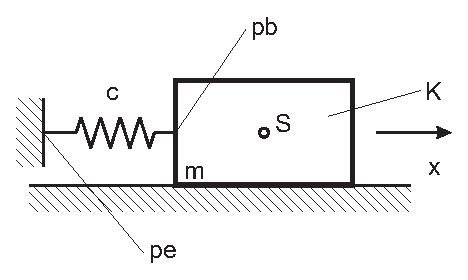
\includegraphics[width=0.45\hsize]{mbsim_one_mass_oscillator.eps}

%%------------------------------------------------------------ SUBSUBSECTION ---------------------
\subsubsection{Physics - system}

\paragraph{Header}

\listinginput{1}{C++/system.h}

\begin{tabular}{r|p{0.85\hsize}}
  1,2,13 & avoids including Header more than once\\
  4,5  & \emph{includes}\\
  7 & class definition for one mass oscillator, which is derived by \texttt{DynamicSystemSolver} without additional functionality\\
  9 & constructor
\end{tabular}

%------------------------------------------------------------
\paragraph{Source}

\listinginput{1}{C++/system.cc}

%%------------------------------------------------------------ SUBSUBSECTION ---------------------
\subsubsection{Time integration -- main}

\listinginput{1}{C++/main.cc}

%%------------------------------------------------------------ SUBSUBSECTION ---------------------
\subsubsection{Makefile} \enlargethispage{5mm}
The building process of a program is controlled by a Makefile:
\listinginput{1}{C++/Makefile}

%%--------------------------------------------------------------- SUBSECTION --
\subsection{2D-Slider Crank Mechanism}
Use the following plan.
\begin{enumerate}
\item rigid bodies with
\begin{itemize}
\item \emph{RigidBody} for crank, pistin and block
\item mass/ length/ width/ inertia tensor
\item Jacobian matrices (translation / rotation)
\item reference frames
\item \OpenMBV{}-bodies (probably one needs an additional translation as \OpenMBV{}-bodies sometimes use another reference)
\end{itemize}

\item elastic connecting rod with
\begin{itemize}
\item \emph{FlexibleBody1s21RCM}
\item length/ width / height (cross-sectional area) / Young's modulus (10e8)/ area moment of inertia / density/ damping
\item number of finite elements
\item reference frames
\item initial generalised coordinates
\end{itemize}

\item frames/ contours in body coordinate system
\item link definition
\item external loads
\item add to dynamic system solver
\item integrator / time step size
\end{enumerate}

%%--------------------------------------------------------------- SUBSECTION --
\subsection{3D-Slider Crank Mechanism}
Use the following plan.
\begin{enumerate}
\item rigid bodies with
\begin{itemize}
\item \emph{RigidBody} for crank, connecting rod, piston and block
\item mass/ length/ width / inertia tensor
\item Jacobian matrices (translation / rotation)
\item reference frames
\item \OpenMBV{}-bodies
\end{itemize}

\item frames / contours in body coordinate system
\item link definition
\item external loads
\item add to dynamic system solver
\item integrator / time step size
\end{enumerate}



\appendix
\section{Trouble-Shooting}
\subsection{GNU-Build-System}\label{sec:gnu}
The role of the GNU-Build-System (Figure \ref{fig:GNUBuild}) 
\begin{figure}[h]
	\centering
	
    \psfrag{acinclude.m4}{\textsf{\small acinclude.m4}}
    \psfrag{aclocal.m4}{\textsf{\small aclocal.m4}}
    \psfrag{aclocal}{\textsf{\small aclocal}}
    \psfrag{configure.ac}{\textsf{\small configure.ac}}
    \psfrag{autoconf}{\textsf{\small autoconf}}
    \psfrag{Makefile.am ...}{\textsf{\small Makefile.am}}
    \psfrag{automake}{\textsf{\small automake}}
    \psfrag{libtoolize}{\textsf{\small libtoolize}}
    \psfrag{Makefile.in ...}{\textsf{\small Makefile.in}}
    \psfrag{configure}{\textsf{\small configure}}
    \psfrag{Legende}{\textsf{\small legend}}
    \psfrag{Eingabe-Datei}{\textsf{\small input file}}
    \psfrag{Ausgabe-Datei}{\textsf{\small output file}}
    \psfrag{Programm}{\textsf{\small program}}
    \psfrag{Skript}{\textsf{\small procedure}}
    \psfrag{make}{\textsf{\small make}}
    \psfrag{Makefile ...}{\textsf{\small Makefile}}
  	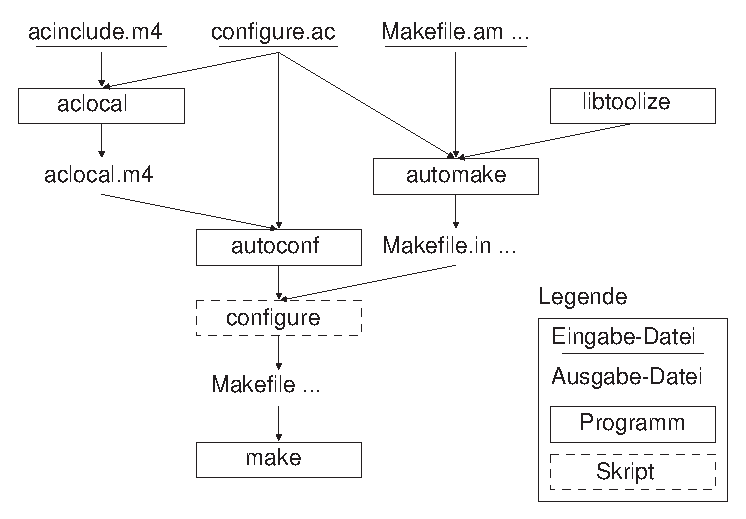
\includegraphics[width=12cm]{Figures/mbsim_gnubuildsystem.eps}
  	\caption{GNU build system}
  	\label{fig:GNUBuild}
\end{figure}
can be summarized as follows.\footnote{in detail: \url{www.gnu.org/software/[autoconf,automake,libtool]/manual}}\par\nopagebreak
	\begin{tabular}{|l|p{100mm}|}
	\hline
		\texttt{aclocal} & Generates M4 macros necessary for the following procedures.\\\hline
		\texttt{autoheader} & Creates \texttt{config.h.in} as basis for header files.\\\hline
		\texttt{autoconf} & Compiler for \texttt{configure.ac} to build the executable \textsc{configure} procedure.\\\hline
		\verb|libtoolize -c --force| & Generates shell and M4 procedures for the system depending shared object files. The option \texttt{-c} forces a local copy of the defining files instead of links. The option \texttt{--force} overwrites already existing procedures.\\\hline
		\texttt{automake -a -c --force} & Compiler for \texttt{Makefile.am} for preparation of \texttt{Makefile.in}. The option \texttt{-c} forces a local copy of the defining files instead of links. The option \texttt{-a} adds missing standard files. The option \texttt{--force} overwrites already existing procedures.\\\hline
		\texttt{autoreconf -fi} & Summarizes \texttt{aclocal}, \texttt{autoheader}, \texttt{autoconf}, \texttt{automake}.\\\hline
		\texttt{make} & Compiles the project sources and links with preliminary libraries. On multi-core computers it is possible to define the number~\texttt{n} of parallel jobs with \texttt{-jn} to accelerate compilation.\\\hline
		\texttt{make install} & Copies the executable project files and \texttt{includes} to \texttt{\$HOME/MBSim/Install}.\\\hline 
        \texttt{./configure} & Invokes system dependent checks and substitutes in existing \texttt{.in}-files variables by systemdepending informationen. The option \texttt{--enable-static --disable-shared} only produces a static build, vice versa a shared library is built. Without such an option normally both shared (*.so) and static (*.a) libraries are provided.\\\hline
	\end{tabular}

\subsection{Third Party Software}\label{sec:third_party}
Necessary for the installation of a static visualisation part are the following preliminary steps with everything being installed by package service or from scratch in \texttt{/home/OpenMBV} with some hints:
\begin{itemize}
\item \texttt{export PKG\_CONFIG\_PATH=/home/OpenMBV/local/lib/pkgconfig}
\item Coin3d with version 3 or newer (3D scenegraphs)\\
    \texttt{./configure --prefix=/home/OpenMBV/local --disable-shared --enable-static}
\item hdf5 with version 1.8.2 or newer (file handling)\\
    \texttt{./configure --prefix=/home/OpenMBV/local --disable-shared --enable-static\\ --enable-cxx --with-zlib=no}
\item Qt with version 4.4 or newer (2D user interface)\\
    \texttt{./configure -prefix /home/OpenMBV/local -static -nomake examples -nomake demos\\ -nomake docs -nomake translations -no-gif -no-libtiff -qt-libpng -no-libmng\\ -qt-libjpeg -no-openssl -no-glib}
\item HDF5Serie (wrapper for file handling)\\
    \texttt{./configure --prefix=/home/OpenMBV/local --disable-shared --enable-static}
\item SoQt with version 1.4.1 or newer (e.g. event invocation in Coin due to hardware events)\\
    \texttt{in SoQtComponent.cpp:103' change "unsinged long key" to "uintptr\_t key"}\\
    \texttt{export QTDIR=/home/OpenMBV/local}\\
    \texttt{export CONFIG\_QTLIBS="\$(pkg-config --libs QtGui QtCore Qt3Support QtOpenGL)"}\\
    \texttt{./configure --prefix=/home/OpenMBV/local --disable-shared --enable-static}
\item Qwt with version 5 or newer (GUI elements)\\
    \texttt{in qwtconfig.pri change INSTALLBASE=/home/OpenMBV/local}\\
    \texttt{/home/OpenMBV/local/bin/qmake}
\item Octave with version 3.0 or newer (for XML preprocessing) 
\end{itemize}

\subsection{Path Information}
After recognising difficulties concerning path information mistakes in the objects should be ruled out by \texttt{make clean}. Then, path information in \texttt{.bashrc} and finally in the affected \texttt{.pc}-files should be checked. The location of the \texttt{.pc}-files can be found by
\begin{verbatim}
pkg-config --cflags mbsim
pkg-config --libs mbsim
\end{verbatim}

\subsection{Often Needed Linux Advices}
\begin{itemize}
\item After editing \texttt{\$HOME/.bashrc} the shell has to be restarted or the command \texttt{source \$HOME/.bashrc} has to be invoked
\end{itemize}

\section{\MBSim{} - Coding Standard}
In the following the Coding standards of \MBSim{} and the associated projects is defined.
\listinginput{1}{mbsimcodingstandard.h}


%%%%%%%%%%%%%%%%%%%%%%%%%%%%%%%%%%%%%%%%%%%%%%%%%%%%%%%%%%%%%%%%%%%%%%%%%%%%%%%%
%%%%%%%%%%%%%%%%%%%%%%%%%%%%%%%%%%%%%%%%%%%%%%%%%%%%%%%%%%%%%%%%%%%%%%%%%%%%%%%%

\bibliographystyle{plain}
\bibliography{Literatur}
\end{document}

